\date{}
\documentclass[12pt]{article}
\usepackage{mathptmx}% http://ctan.org/pkg/mathptmx
\usepackage{graphicx}
\usepackage{lscape}
\usepackage{rotating}
\usepackage[top=1.5cm, bottom=2.2cm, left=3cm, right=2cm, headsep=1.2cm, footskip=1cm, headheight=0.3cm, textheight=24.5cm, textwidth=16cm]{geometry}
\usepackage{fancyhdr}
\makeatletter
\def\@seccntformat#1{%
  \expandafter\ifx\csname c@#1\endcsname\c@section\else
  \csname the#1\endcsname\quad
  \fi}
\makeatother
\renewcommand{\baselinestretch}{1.5}
\title{\textbf{Chapter 4}\vspace{-6ex}}

\begin{document}
\maketitle

\pagenumbering{arabic}
\setcounter{page}{13}

\begin{center}
\section{Analysis Modeling}
\end{center}

\setcounter{section}{4}

\subsection{Functional Modeling}\newline
\textbf{Data Flow Diagram}\newline
Data flow diagrams provide a graphical representation of how information moves between processes in a system. A Data Flow Diagram shows what kind of information will be input to and output from the system, where the data will come from and go to, and where the data will be stored.\newline

\noindent\underline{\textbf{Level 0 DFD for detecting phishing websites using data mining}}\newline

\begin{figure}[h]
\centering
\graphicspath{ Diagrams/ }
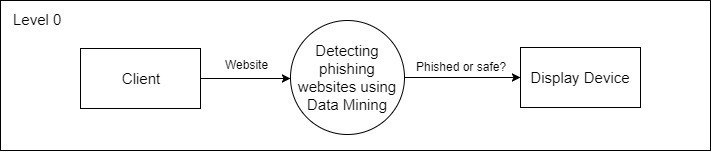
\includegraphics[scale=0.6]{Diagrams/DFD_level_0.jpg}
\setcounter{figure}{0}
\renewcommand{\thefigure}{\arabic{section}.\arabic{subsection}.\arabic{figure}}
\caption{DFD Level 0}
\end{figure}\newline

In this level 0 data flow diagram, the whole system is represented with the help of input, processing and output. The input to system is the URL entered by the end user. The system should display appropriate alert on the web browser if a phished website is detected. \newline

\newgeometry{top=3cm, bottom=2.2cm, left=3cm, right=2cm, headsep=1.2cm, footskip=1cm, headheight=0.3cm, textheight=24.5cm, textwidth=16cm}

\pagestyle{fancy}
\renewcommand{\headrulewidth}{0pt}
\lhead{Chapter 4}
\rhead{Analysis Modeling}

\noindent\underline{\textbf{Level 1 DFD for detecting phishing websites using data mining}}\newline

\begin{figure}[h]
\centering
\graphicspath{ Diagrams/ }
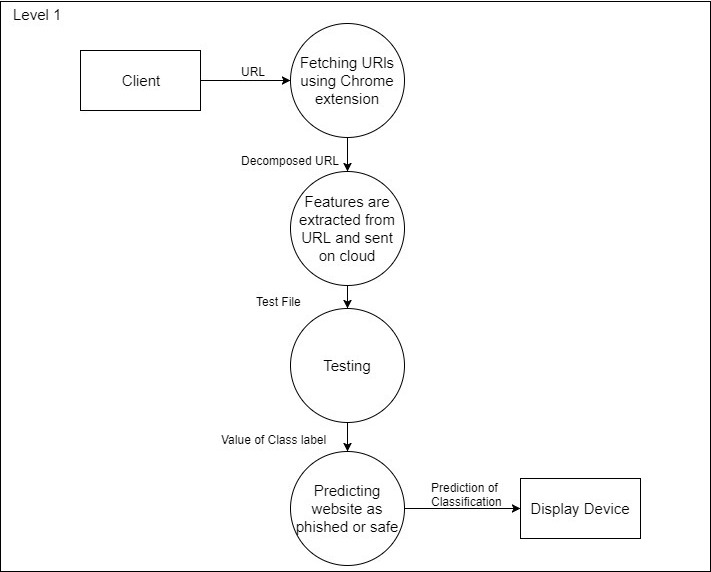
\includegraphics[scale=0.6]{Diagrams/DFD_level_1.jpg}
\setcounter{figure}{1}
\renewcommand{\thefigure}{\arabic{section}.\arabic{subsection}.\arabic{figure}}
\caption{DFD Level 1}
\end{figure}\newline

In level 1 data flow diagram, we have shown the process for phishing detection. When the client visits the URL, the Chrome extension will fetch the URL. The URL attributes are then extracted from the URL by the Chrome extension. These features are used as test data. Based on this, classifier predicts the website as safe or phished.\newline

\newgeometry{top=3cm, bottom=2.2cm, left=3cm, right=2cm, headsep=1.2cm, footskip=1cm, headheight=0.3cm, textheight=24.5cm, textwidth=16cm}

\pagestyle{fancy}
\renewcommand{\headrulewidth}{0pt}
\lhead{4.1}
\rhead{Functional Modeling}

\noindent\underline{\textbf{Level 2 DFD for detecting phishing websites using data mining}}
\begin{figure}[h]
\centering
\graphicspath{ Diagrams/ }
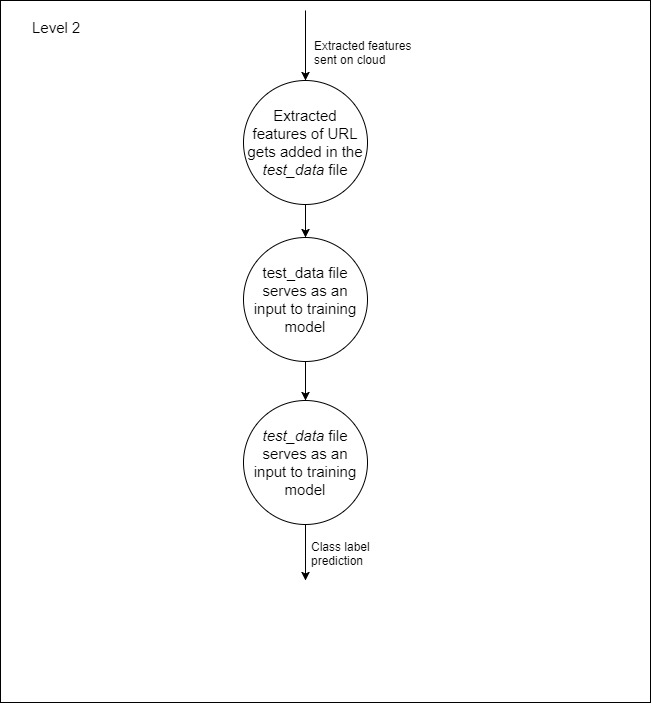
\includegraphics[scale=0.6]{Diagrams/DFD_level_2.jpg}
\setcounter{figure}{2}
\renewcommand{\thefigure}{\arabic{section}.\arabic{subsection}.\arabic{figure}}
\caption{DFD Level 2}
\end{figure}


In level 2 data flow diagram, we have shown the detailed testing process. When the Chrome extension extracts the URL features, a test data file is created where the extracted URL attributes are added. (Each time a user visits a URL, a new \textit{test data} file will be created which will only contain the visited URL as a \textit{test data}). This file is then sent on the cloud for testing. The \textit{test data} file acts as an input to the trained model. The model will then predict the value of the class label, which predicts the website as safe or phished. If the website is phished, the alert message is given to the user.

\newgeometry{top=3cm, bottom=2.2cm, left=3cm, right=2cm, headsep=1.2cm, footskip=1cm, headheight=0.3cm, textheight=24.5cm, textwidth=16cm}

\pagestyle{fancy}
\renewcommand{\headrulewidth}{0pt}
\lhead{Chapter 4}
\rhead{Analysis Modeling}

\subsection{Activity Diagram:}\newline

\begin{figure}[h]
\centering
\graphicspath{ Diagrams/ }
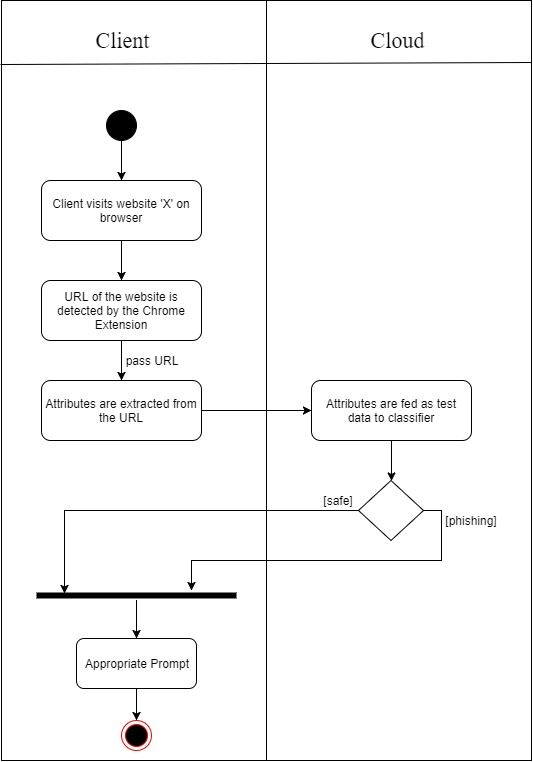
\includegraphics[scale=0.6]{Diagrams/Activity_Diagram.jpg}
\setcounter{figure}{0}
\renewcommand{\thefigure}{\arabic{section}.\arabic{subsection}.\arabic{figure}}
\caption{Activity Diagram}
\end{figure}

In figure 4.2, we have shown the activity diagram for Detecting Phishing websites using Data Mining. It is divided into client side and cloud side, thereby segregating the tasks for both. The client visits the website. The chrome extension on web browser fetches the URL and extracts the attributes from it. These attributes are sent on cloud where it is tested by the trained model residing on the cloud.

\newgeometry{top=3cm, bottom=2.2cm, left=3cm, right=2cm, headsep=1.2cm, footskip=1cm, headheight=0.3cm, textheight=24.5cm, textwidth=16cm}

\pagestyle{fancy}
\renewcommand{\headrulewidth}{0pt}
\lhead{4.3}
\rhead{Flowchart}

\subsection{Flowchart:}

\begin{figure}[h]
\centering
\graphicspath{ Diagrams/ }
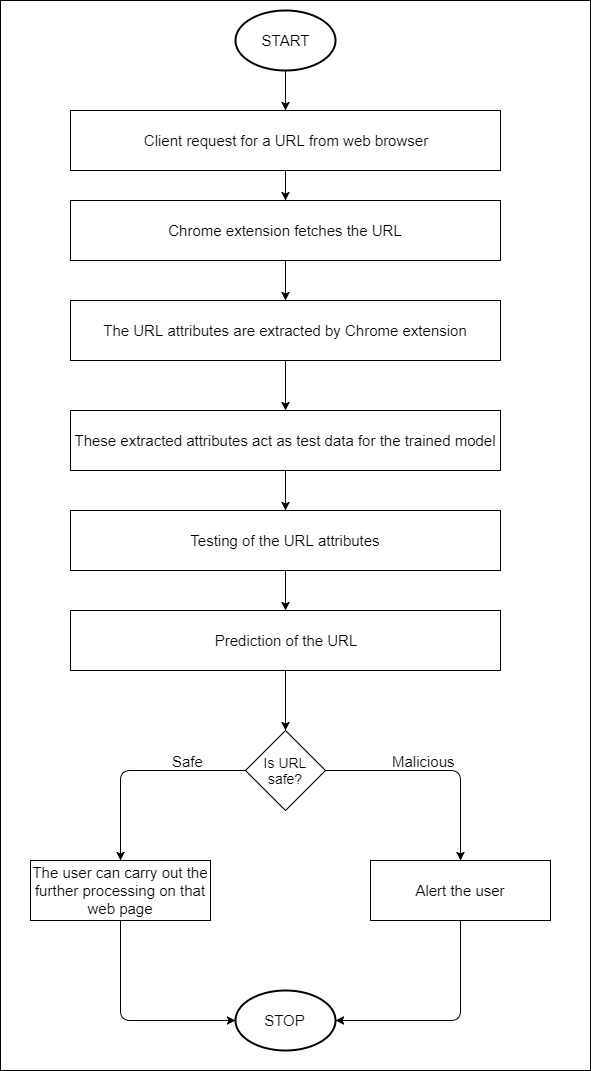
\includegraphics[scale=0.4]{Diagrams/flowchart.jpg}
\setcounter{figure}{0}
\renewcommand{\thefigure}{\arabic{section}.\arabic{subsection}.\arabic{figure}}
\caption{Flowchart for Phishing Detection using Data Mining}
\end{figure}

In figure 4.3.1, we have shown the complete flow of the project. To start with, the client visits a URL. As soon as the client visits the URL, the chrome extension on user’s browser will fetch that URL and extract the attributes of the URL. These attributes are then sent on the cloud where the classifier is deployed. The trained model then performs the testing of these URL attributes and predicts the legitimacy of the URL. It then alerts the user regarding the same. It is up to the user to proceed even if we alert about the phished website.

\newgeometry{top=3cm, bottom=2.2cm, left=3cm, right=2cm, headsep=1.2cm, footskip=1cm, headheight=0.3cm, textheight=24.5cm, textwidth=16cm}

\pagestyle{fancy}
\renewcommand{\headrulewidth}{0pt}
\lhead{Chapter 4}
\rhead{Analysis Modeling}

\subsection{Timeline Chart:}

\begin{figure}[h]
\centering
\graphicspath{ Diagrams/ }
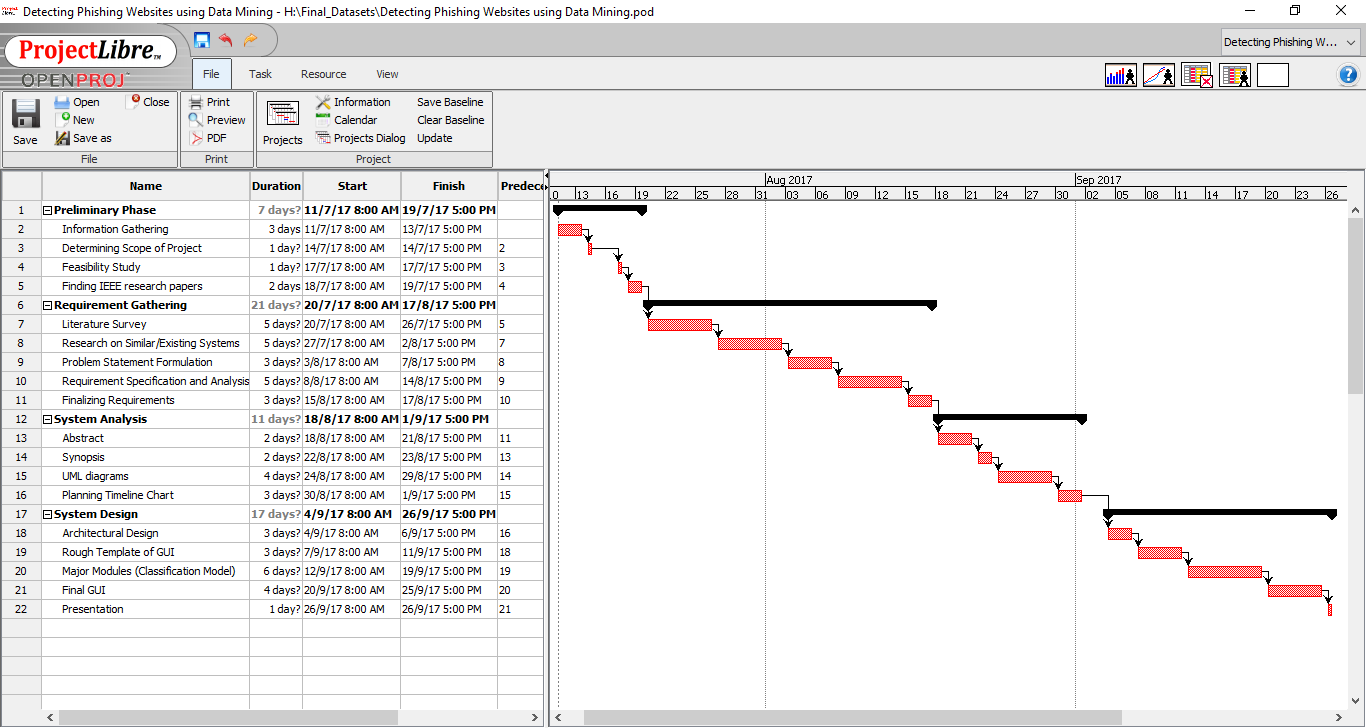
\includegraphics[width=16cm,height=9cm,angle=90]{Diagrams/GanttChartCombinedFinal.png}
\setcounter{figure}{0}
\renewcommand{\thefigure}{\arabic{section}.\arabic{subsection}.\arabic{figure}}
\caption{Timeline chart}
\end{figure}\newline

\newgeometry{top=3cm, bottom=2.2cm, left=3cm, right=2cm, headsep=1.2cm, footskip=1cm, headheight=0.3cm, textheight=24.5cm, textwidth=16cm}

\pagestyle{fancy}
\renewcommand{\headrulewidth}{0pt}
\lhead{4.4}
\rhead{Timeline Chart}

Good planning spreads the necessary work over a reasonable period of time and allows everyone to work at a consistent, sustainable pace. 
A Timeline is a clean and concise visual representation of a series of events. It helps to arrange large chunks of time and see the overall plan easily. A timeline is typically divided into chunks, each ending with a milestone.\newline

\noindent Here we have shown the Timeline chart, which shows the basic schedule of our project. The project has been divided into the phases and sub phases. The corresponding Gantt chart is also shown which gives an idea as to which phase has to be given more time.\newline
\end{document}